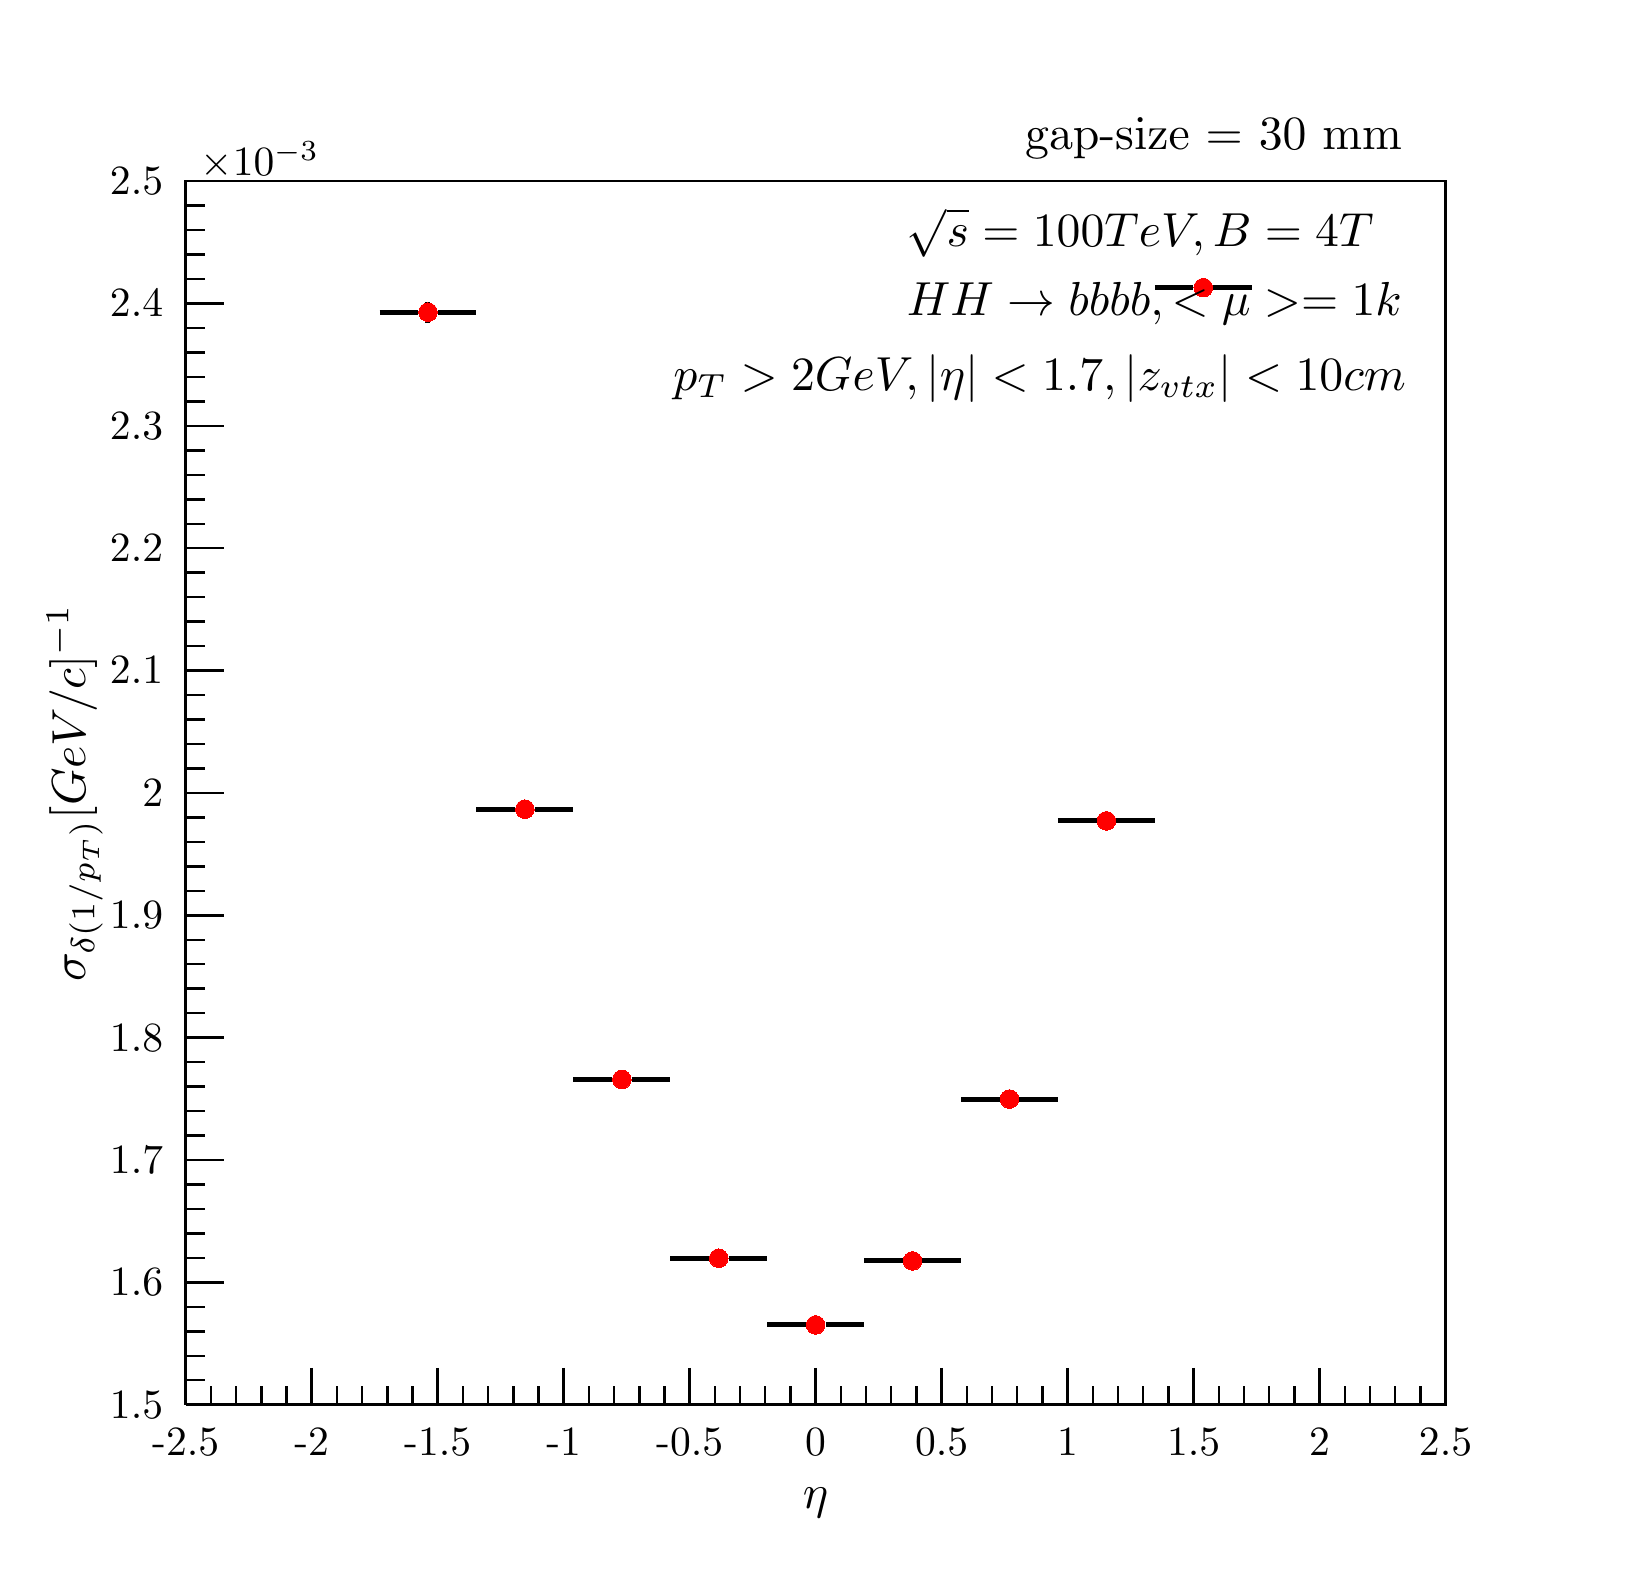
\begin{tikzpicture}
\pgfdeclareplotmark{cross} {
\pgfpathmoveto{\pgfpoint{-0.3\pgfplotmarksize}{\pgfplotmarksize}}
\pgfpathlineto{\pgfpoint{+0.3\pgfplotmarksize}{\pgfplotmarksize}}
\pgfpathlineto{\pgfpoint{+0.3\pgfplotmarksize}{0.3\pgfplotmarksize}}
\pgfpathlineto{\pgfpoint{+1\pgfplotmarksize}{0.3\pgfplotmarksize}}
\pgfpathlineto{\pgfpoint{+1\pgfplotmarksize}{-0.3\pgfplotmarksize}}
\pgfpathlineto{\pgfpoint{+0.3\pgfplotmarksize}{-0.3\pgfplotmarksize}}
\pgfpathlineto{\pgfpoint{+0.3\pgfplotmarksize}{-1.\pgfplotmarksize}}
\pgfpathlineto{\pgfpoint{-0.3\pgfplotmarksize}{-1.\pgfplotmarksize}}
\pgfpathlineto{\pgfpoint{-0.3\pgfplotmarksize}{-0.3\pgfplotmarksize}}
\pgfpathlineto{\pgfpoint{-1.\pgfplotmarksize}{-0.3\pgfplotmarksize}}
\pgfpathlineto{\pgfpoint{-1.\pgfplotmarksize}{0.3\pgfplotmarksize}}
\pgfpathlineto{\pgfpoint{-0.3\pgfplotmarksize}{0.3\pgfplotmarksize}}
\pgfpathclose
\pgfusepathqstroke
}
\pgfdeclareplotmark{cross*} {
\pgfpathmoveto{\pgfpoint{-0.3\pgfplotmarksize}{\pgfplotmarksize}}
\pgfpathlineto{\pgfpoint{+0.3\pgfplotmarksize}{\pgfplotmarksize}}
\pgfpathlineto{\pgfpoint{+0.3\pgfplotmarksize}{0.3\pgfplotmarksize}}
\pgfpathlineto{\pgfpoint{+1\pgfplotmarksize}{0.3\pgfplotmarksize}}
\pgfpathlineto{\pgfpoint{+1\pgfplotmarksize}{-0.3\pgfplotmarksize}}
\pgfpathlineto{\pgfpoint{+0.3\pgfplotmarksize}{-0.3\pgfplotmarksize}}
\pgfpathlineto{\pgfpoint{+0.3\pgfplotmarksize}{-1.\pgfplotmarksize}}
\pgfpathlineto{\pgfpoint{-0.3\pgfplotmarksize}{-1.\pgfplotmarksize}}
\pgfpathlineto{\pgfpoint{-0.3\pgfplotmarksize}{-0.3\pgfplotmarksize}}
\pgfpathlineto{\pgfpoint{-1.\pgfplotmarksize}{-0.3\pgfplotmarksize}}
\pgfpathlineto{\pgfpoint{-1.\pgfplotmarksize}{0.3\pgfplotmarksize}}
\pgfpathlineto{\pgfpoint{-0.3\pgfplotmarksize}{0.3\pgfplotmarksize}}
\pgfpathclose
\pgfusepathqfillstroke
}
\pgfdeclareplotmark{newstar} {
\pgfpathmoveto{\pgfqpoint{0pt}{\pgfplotmarksize}}
\pgfpathlineto{\pgfqpointpolar{44}{0.5\pgfplotmarksize}}
\pgfpathlineto{\pgfqpointpolar{18}{\pgfplotmarksize}}
\pgfpathlineto{\pgfqpointpolar{-20}{0.5\pgfplotmarksize}}
\pgfpathlineto{\pgfqpointpolar{-54}{\pgfplotmarksize}}
\pgfpathlineto{\pgfqpointpolar{-90}{0.5\pgfplotmarksize}}
\pgfpathlineto{\pgfqpointpolar{234}{\pgfplotmarksize}}
\pgfpathlineto{\pgfqpointpolar{198}{0.5\pgfplotmarksize}}
\pgfpathlineto{\pgfqpointpolar{162}{\pgfplotmarksize}}
\pgfpathlineto{\pgfqpointpolar{134}{0.5\pgfplotmarksize}}
\pgfpathclose
\pgfusepathqstroke
}
\pgfdeclareplotmark{newstar*} {
\pgfpathmoveto{\pgfqpoint{0pt}{\pgfplotmarksize}}
\pgfpathlineto{\pgfqpointpolar{44}{0.5\pgfplotmarksize}}
\pgfpathlineto{\pgfqpointpolar{18}{\pgfplotmarksize}}
\pgfpathlineto{\pgfqpointpolar{-20}{0.5\pgfplotmarksize}}
\pgfpathlineto{\pgfqpointpolar{-54}{\pgfplotmarksize}}
\pgfpathlineto{\pgfqpointpolar{-90}{0.5\pgfplotmarksize}}
\pgfpathlineto{\pgfqpointpolar{234}{\pgfplotmarksize}}
\pgfpathlineto{\pgfqpointpolar{198}{0.5\pgfplotmarksize}}
\pgfpathlineto{\pgfqpointpolar{162}{\pgfplotmarksize}}
\pgfpathlineto{\pgfqpointpolar{134}{0.5\pgfplotmarksize}}
\pgfpathclose
\pgfusepathqfillstroke
}
\definecolor{c}{rgb}{1,1,1};
\draw [color=c, fill=c] (0,0) rectangle (20,19.4236);
\draw [color=c, fill=c] (2,1.94236) rectangle (18,17.4812);
\definecolor{c}{rgb}{0,0,0};
\draw [c,line width=0.9] (2,1.94236) -- (2,17.4812) -- (18,17.4812) -- (18,1.94236) -- (2,1.94236);
\definecolor{c}{rgb}{1,1,1};
\draw [color=c, fill=c] (2,1.94236) rectangle (18,17.4812);
\definecolor{c}{rgb}{0,0,0};
\draw [c,line width=0.9] (2,1.94236) -- (2,17.4812) -- (18,17.4812) -- (18,1.94236) -- (2,1.94236);
\draw [c,line width=1.8] (5.07692,15.6908) -- (5.07692,15.6918);
\draw [c,line width=1.8] (5.07692,15.9424) -- (5.07692,15.9434);
\draw [c,line width=1.8] (4.46154,15.8171) -- (4.95161,15.8171);
\draw [c,line width=1.8] (5.20224,15.8171) -- (5.69231,15.8171);
\definecolor{c}{rgb}{1,0,0};
\foreach \P in {(5.07692,15.8171)}{\draw[mark options={color=c,fill=c},mark size=3.363363pt, line width=0.000000pt, mark=*] plot coordinates {\P};}
\definecolor{c}{rgb}{0,0,0};
\draw [c,line width=1.8] (5.69231,9.50594) -- (6.18238,9.50594);
\draw [c,line width=1.8] (6.43301,9.50594) -- (6.92308,9.50594);
\definecolor{c}{rgb}{1,0,0};
\foreach \P in {(6.30769,9.50594)}{\draw[mark options={color=c,fill=c},mark size=3.363363pt, line width=0.000000pt, mark=*] plot coordinates {\P};}
\definecolor{c}{rgb}{0,0,0};
\draw [c,line width=1.8] (6.92308,6.07261) -- (7.41315,6.07261);
\draw [c,line width=1.8] (7.66377,6.07261) -- (8.15385,6.07261);
\definecolor{c}{rgb}{1,0,0};
\foreach \P in {(7.53846,6.07261)}{\draw[mark options={color=c,fill=c},mark size=3.363363pt, line width=0.000000pt, mark=*] plot coordinates {\P};}
\definecolor{c}{rgb}{0,0,0};
\draw [c,line width=1.8] (8.15385,3.80238) -- (8.64392,3.80238);
\draw [c,line width=1.8] (8.89454,3.80238) -- (9.38461,3.80238);
\definecolor{c}{rgb}{1,0,0};
\foreach \P in {(8.76923,3.80238)}{\draw[mark options={color=c,fill=c},mark size=3.363363pt, line width=0.000000pt, mark=*] plot coordinates {\P};}
\definecolor{c}{rgb}{0,0,0};
\draw [c,line width=1.8] (9.38461,2.95542) -- (9.87469,2.95542);
\draw [c,line width=1.8] (10.1253,2.95542) -- (10.6154,2.95542);
\definecolor{c}{rgb}{1,0,0};
\foreach \P in {(10,2.95542)}{\draw[mark options={color=c,fill=c},mark size=3.363363pt, line width=0.000000pt, mark=*] plot coordinates {\P};}
\definecolor{c}{rgb}{0,0,0};
\draw [c,line width=1.8] (10.6154,3.76754) -- (11.1055,3.76754);
\draw [c,line width=1.8] (11.3561,3.76754) -- (11.8462,3.76754);
\definecolor{c}{rgb}{1,0,0};
\foreach \P in {(11.2308,3.76754)}{\draw[mark options={color=c,fill=c},mark size=3.363363pt, line width=0.000000pt, mark=*] plot coordinates {\P};}
\definecolor{c}{rgb}{0,0,0};
\draw [c,line width=1.8] (11.8462,5.82448) -- (12.3362,5.82448);
\draw [c,line width=1.8] (12.5869,5.82448) -- (13.0769,5.82448);
\definecolor{c}{rgb}{1,0,0};
\foreach \P in {(12.4615,5.82448)}{\draw[mark options={color=c,fill=c},mark size=3.363363pt, line width=0.000000pt, mark=*] plot coordinates {\P};}
\definecolor{c}{rgb}{0,0,0};
\draw [c,line width=1.8] (13.0769,9.35701) -- (13.567,9.35701);
\draw [c,line width=1.8] (13.8176,9.35701) -- (14.3077,9.35701);
\definecolor{c}{rgb}{1,0,0};
\foreach \P in {(13.6923,9.35701)}{\draw[mark options={color=c,fill=c},mark size=3.363363pt, line width=0.000000pt, mark=*] plot coordinates {\P};}
\definecolor{c}{rgb}{0,0,0};
\draw [c,line width=1.8] (14.3077,16.1288) -- (14.7978,16.1288);
\draw [c,line width=1.8] (15.0484,16.1288) -- (15.5385,16.1288);
\definecolor{c}{rgb}{1,0,0};
\foreach \P in {(14.9231,16.1288)}{\draw[mark options={color=c,fill=c},mark size=3.363363pt, line width=0.000000pt, mark=*] plot coordinates {\P};}
\definecolor{c}{rgb}{0,0,0};
\draw [c,line width=0.9] (2,1.94236) -- (18,1.94236);
\draw [c,line width=0.9] (2,2.40852) -- (2,1.94236);
\draw [c,line width=0.9] (2.32,2.17544) -- (2.32,1.94236);
\draw [c,line width=0.9] (2.64,2.17544) -- (2.64,1.94236);
\draw [c,line width=0.9] (2.96,2.17544) -- (2.96,1.94236);
\draw [c,line width=0.9] (3.28,2.17544) -- (3.28,1.94236);
\draw [c,line width=0.9] (3.6,2.40852) -- (3.6,1.94236);
\draw [c,line width=0.9] (3.92,2.17544) -- (3.92,1.94236);
\draw [c,line width=0.9] (4.24,2.17544) -- (4.24,1.94236);
\draw [c,line width=0.9] (4.56,2.17544) -- (4.56,1.94236);
\draw [c,line width=0.9] (4.88,2.17544) -- (4.88,1.94236);
\draw [c,line width=0.9] (5.2,2.40852) -- (5.2,1.94236);
\draw [c,line width=0.9] (5.52,2.17544) -- (5.52,1.94236);
\draw [c,line width=0.9] (5.84,2.17544) -- (5.84,1.94236);
\draw [c,line width=0.9] (6.16,2.17544) -- (6.16,1.94236);
\draw [c,line width=0.9] (6.48,2.17544) -- (6.48,1.94236);
\draw [c,line width=0.9] (6.8,2.40852) -- (6.8,1.94236);
\draw [c,line width=0.9] (7.12,2.17544) -- (7.12,1.94236);
\draw [c,line width=0.9] (7.44,2.17544) -- (7.44,1.94236);
\draw [c,line width=0.9] (7.76,2.17544) -- (7.76,1.94236);
\draw [c,line width=0.9] (8.08,2.17544) -- (8.08,1.94236);
\draw [c,line width=0.9] (8.4,2.40852) -- (8.4,1.94236);
\draw [c,line width=0.9] (8.72,2.17544) -- (8.72,1.94236);
\draw [c,line width=0.9] (9.04,2.17544) -- (9.04,1.94236);
\draw [c,line width=0.9] (9.36,2.17544) -- (9.36,1.94236);
\draw [c,line width=0.9] (9.68,2.17544) -- (9.68,1.94236);
\draw [c,line width=0.9] (10,2.40852) -- (10,1.94236);
\draw [c,line width=0.9] (10.32,2.17544) -- (10.32,1.94236);
\draw [c,line width=0.9] (10.64,2.17544) -- (10.64,1.94236);
\draw [c,line width=0.9] (10.96,2.17544) -- (10.96,1.94236);
\draw [c,line width=0.9] (11.28,2.17544) -- (11.28,1.94236);
\draw [c,line width=0.9] (11.6,2.40852) -- (11.6,1.94236);
\draw [c,line width=0.9] (11.92,2.17544) -- (11.92,1.94236);
\draw [c,line width=0.9] (12.24,2.17544) -- (12.24,1.94236);
\draw [c,line width=0.9] (12.56,2.17544) -- (12.56,1.94236);
\draw [c,line width=0.9] (12.88,2.17544) -- (12.88,1.94236);
\draw [c,line width=0.9] (13.2,2.40852) -- (13.2,1.94236);
\draw [c,line width=0.9] (13.52,2.17544) -- (13.52,1.94236);
\draw [c,line width=0.9] (13.84,2.17544) -- (13.84,1.94236);
\draw [c,line width=0.9] (14.16,2.17544) -- (14.16,1.94236);
\draw [c,line width=0.9] (14.48,2.17544) -- (14.48,1.94236);
\draw [c,line width=0.9] (14.8,2.40852) -- (14.8,1.94236);
\draw [c,line width=0.9] (15.12,2.17544) -- (15.12,1.94236);
\draw [c,line width=0.9] (15.44,2.17544) -- (15.44,1.94236);
\draw [c,line width=0.9] (15.76,2.17544) -- (15.76,1.94236);
\draw [c,line width=0.9] (16.08,2.17544) -- (16.08,1.94236);
\draw [c,line width=0.9] (16.4,2.40852) -- (16.4,1.94236);
\draw [c,line width=0.9] (16.72,2.17544) -- (16.72,1.94236);
\draw [c,line width=0.9] (17.04,2.17544) -- (17.04,1.94236);
\draw [c,line width=0.9] (17.36,2.17544) -- (17.36,1.94236);
\draw [c,line width=0.9] (17.68,2.17544) -- (17.68,1.94236);
\draw [c,line width=0.9] (18,2.40852) -- (18,1.94236);
\draw [c,line width=0.9] (18,2.40852) -- (18,1.94236);
\draw [anchor=base] (2,1.30138) node[scale=1.50291, color=c, rotate=0]{-2.5};
\draw [anchor=base] (3.6,1.30138) node[scale=1.50291, color=c, rotate=0]{-2};
\draw [anchor=base] (5.2,1.30138) node[scale=1.50291, color=c, rotate=0]{-1.5};
\draw [anchor=base] (6.8,1.30138) node[scale=1.50291, color=c, rotate=0]{-1};
\draw [anchor=base] (8.4,1.30138) node[scale=1.50291, color=c, rotate=0]{-0.5};
\draw [anchor=base] (10,1.30138) node[scale=1.50291, color=c, rotate=0]{0};
\draw [anchor=base] (11.6,1.30138) node[scale=1.50291, color=c, rotate=0]{0.5};
\draw [anchor=base] (13.2,1.30138) node[scale=1.50291, color=c, rotate=0]{1};
\draw [anchor=base] (14.8,1.30138) node[scale=1.50291, color=c, rotate=0]{1.5};
\draw [anchor=base] (16.4,1.30138) node[scale=1.50291, color=c, rotate=0]{2};
\draw [anchor=base] (18,1.30138) node[scale=1.50291, color=c, rotate=0]{2.5};
\draw (10,0.699248) node[scale=1.72557, color=c, rotate=0]{$\eta$};
\draw [c,line width=0.9] (2,1.94236) -- (2,17.4812);
\draw [c,line width=0.9] (2.48,1.94236) -- (2,1.94236);
\draw [c,line width=0.9] (2.24,2.25313) -- (2,2.25313);
\draw [c,line width=0.9] (2.24,2.56391) -- (2,2.56391);
\draw [c,line width=0.9] (2.24,2.87469) -- (2,2.87469);
\draw [c,line width=0.9] (2.24,3.18546) -- (2,3.18546);
\draw [c,line width=0.9] (2.48,3.49624) -- (2,3.49624);
\draw [c,line width=0.9] (2.24,3.80702) -- (2,3.80702);
\draw [c,line width=0.9] (2.24,4.11779) -- (2,4.11779);
\draw [c,line width=0.9] (2.24,4.42857) -- (2,4.42857);
\draw [c,line width=0.9] (2.24,4.73935) -- (2,4.73935);
\draw [c,line width=0.9] (2.48,5.05013) -- (2,5.05013);
\draw [c,line width=0.9] (2.24,5.3609) -- (2,5.3609);
\draw [c,line width=0.9] (2.24,5.67168) -- (2,5.67168);
\draw [c,line width=0.9] (2.24,5.98246) -- (2,5.98246);
\draw [c,line width=0.9] (2.24,6.29323) -- (2,6.29323);
\draw [c,line width=0.9] (2.48,6.60401) -- (2,6.60401);
\draw [c,line width=0.9] (2.24,6.91479) -- (2,6.91479);
\draw [c,line width=0.9] (2.24,7.22556) -- (2,7.22556);
\draw [c,line width=0.9] (2.24,7.53634) -- (2,7.53634);
\draw [c,line width=0.9] (2.24,7.84712) -- (2,7.84712);
\draw [c,line width=0.9] (2.48,8.1579) -- (2,8.1579);
\draw [c,line width=0.9] (2.24,8.46867) -- (2,8.46867);
\draw [c,line width=0.9] (2.24,8.77945) -- (2,8.77945);
\draw [c,line width=0.9] (2.24,9.09023) -- (2,9.09023);
\draw [c,line width=0.9] (2.24,9.401) -- (2,9.401);
\draw [c,line width=0.9] (2.48,9.71178) -- (2,9.71178);
\draw [c,line width=0.9] (2.24,10.0226) -- (2,10.0226);
\draw [c,line width=0.9] (2.24,10.3333) -- (2,10.3333);
\draw [c,line width=0.9] (2.24,10.6441) -- (2,10.6441);
\draw [c,line width=0.9] (2.24,10.9549) -- (2,10.9549);
\draw [c,line width=0.9] (2.48,11.2657) -- (2,11.2657);
\draw [c,line width=0.9] (2.24,11.5764) -- (2,11.5764);
\draw [c,line width=0.9] (2.24,11.8872) -- (2,11.8872);
\draw [c,line width=0.9] (2.24,12.198) -- (2,12.198);
\draw [c,line width=0.9] (2.24,12.5088) -- (2,12.5088);
\draw [c,line width=0.9] (2.48,12.8195) -- (2,12.8195);
\draw [c,line width=0.9] (2.24,13.1303) -- (2,13.1303);
\draw [c,line width=0.9] (2.24,13.4411) -- (2,13.4411);
\draw [c,line width=0.9] (2.24,13.7519) -- (2,13.7519);
\draw [c,line width=0.9] (2.24,14.0627) -- (2,14.0627);
\draw [c,line width=0.9] (2.48,14.3734) -- (2,14.3734);
\draw [c,line width=0.9] (2.24,14.6842) -- (2,14.6842);
\draw [c,line width=0.9] (2.24,14.995) -- (2,14.995);
\draw [c,line width=0.9] (2.24,15.3058) -- (2,15.3058);
\draw [c,line width=0.9] (2.24,15.6165) -- (2,15.6165);
\draw [c,line width=0.9] (2.48,15.9273) -- (2,15.9273);
\draw [c,line width=0.9] (2.24,16.2381) -- (2,16.2381);
\draw [c,line width=0.9] (2.24,16.5489) -- (2,16.5489);
\draw [c,line width=0.9] (2.24,16.8596) -- (2,16.8596);
\draw [c,line width=0.9] (2.24,17.1704) -- (2,17.1704);
\draw [c,line width=0.9] (2.48,17.4812) -- (2,17.4812);
\draw [c,line width=0.9] (2.48,17.4812) -- (2,17.4812);
\draw [anchor= east] (1.9,1.94236) node[scale=1.50291, color=c, rotate=0]{1.5};
\draw [anchor= east] (1.9,3.49624) node[scale=1.50291, color=c, rotate=0]{1.6};
\draw [anchor= east] (1.9,5.05013) node[scale=1.50291, color=c, rotate=0]{1.7};
\draw [anchor= east] (1.9,6.60401) node[scale=1.50291, color=c, rotate=0]{1.8};
\draw [anchor= east] (1.9,8.1579) node[scale=1.50291, color=c, rotate=0]{1.9};
\draw [anchor= east] (1.9,9.71178) node[scale=1.50291, color=c, rotate=0]{2};
\draw [anchor= east] (1.9,11.2657) node[scale=1.50291, color=c, rotate=0]{2.1};
\draw [anchor= east] (1.9,12.8195) node[scale=1.50291, color=c, rotate=0]{2.2};
\draw [anchor= east] (1.9,14.3734) node[scale=1.50291, color=c, rotate=0]{2.3};
\draw [anchor= east] (1.9,15.9273) node[scale=1.50291, color=c, rotate=0]{2.4};
\draw [anchor= east] (1.9,17.4812) node[scale=1.50291, color=c, rotate=0]{2.5};
\draw [anchor=base west] (2,17.5492) node[scale=1.50291, color=c, rotate=0]{$\times10^{-3}$};
\draw (0.592,9.71178) node[scale=1.72557, color=c, rotate=90]{$\sigma_{\delta(1/p_{T})} [GeV/c]^{-1}$};
\draw [anchor=base west] (10.945,16.6533) node[scale=1.72557, color=c, rotate=0]{$\sqrt{s} = 100 TeV, B = 4T$};
\draw [anchor=base west] (10.945,15.7792) node[scale=1.72557, color=c, rotate=0]{$HH \rightarrow b\wwbar{b}b\wwbar{b}, <\mu> = 1k$};
\draw [anchor=base east] (17.7105,14.8241) node[scale=1.72557, color=c, rotate=0]{$p_{T} > 2GeV, |\eta| < 1.7, |z_{vtx}| < 10cm$};
\draw [anchor=base west] (12.445,17.8891) node[scale=1.72557, color=c, rotate=0]{gap-size = 30 mm};
\draw [anchor=base west] (12.445,17.5006) node[scale=1.72557, color=c, rotate=0]{ };
\end{tikzpicture}
